\subsection{Análisis \texorpdfstring{\acs{DAR}}{DAR}}\label{subsec:dar-analisis}

Con los criterios de evaluación definidos y las alternativas tecnológicas identificadas, se realizó el análisis \ac{DAR}. Para ello, se empleó una plantilla de evaluación que permitió valorar sistemáticamente cada alternativa frente a los criterios establecidos. Las tecnologías fueron evaluadas de acuerdo con su nivel de cumplimiento para cada criterio, considerando una escala de valoración de 0 a 5 y la ponderación asignada según la importancia de cada criterio para el proyecto.

Los resultados del análisis \ac{DAR} se presentan en la \autoref{fig:dar}, donde se consolidan las valoraciones obtenidas por las cinco alternativas consideradas: OpenLDAP, 389 Directory Server, ApacheDS, OpenDJ y FreeIPA. A partir de estas valoraciones y sus respectivas ponderaciones se obtuvo la puntuación total de cada alternativa, permitiendo realizar la comparación y determinar cuál presentó la mayor correspondencia con los criterios establecidos.

\begin{figure}[H]
	\centering
	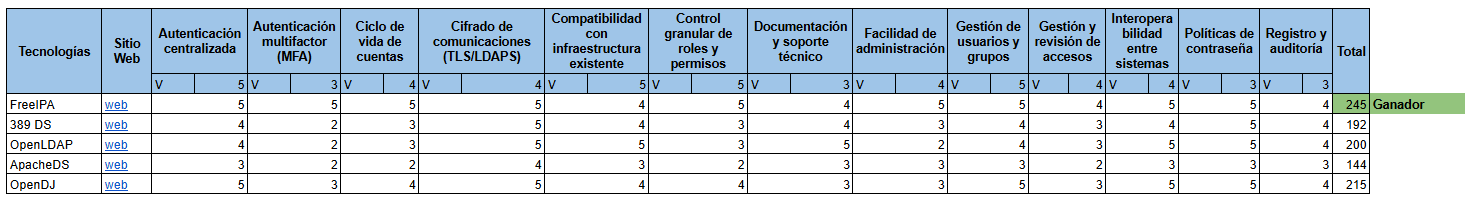
\includegraphics[width=\textwidth]{mainmatter/II-desarrollo-metodologico/dar/imagenes/dar.png}
	\caption{Resultados del análisis \acs{DAR} de las alternativas tecnológicas evaluadas}
	\label{fig:dar}
\end{figure}
